%
%  This document contains chapter 3 of the thesis.
%

\chapter{RESULTS}\label{ch:results}
This chapter attempts to answer the questions previously outlined in the
\hyperref[subsec:analysis]{Analysis} section.
Each section is dedicated to exploring one question.
The process used is described in each section though the process usually
consists of using a combination of graphing, One-way ANOVA tests, and
Student's t- or Mann-Whitney U-tests.
All tests are performed with $\alpha = 0.05$ unless otherwise stated.


\section{Lowest Error Voting Mechanisms}\label{sec:lowest-error-voting-mechanism}
Voting mechanisms consolidate the votes of all agents along with their weights
into a final estimate, and so play a pivotal role in the accuracy of a system.
\autoref{fig:voting-mechanisms-comparison} illustrates the population of
squared error for each voting mechanism.

\begin{figure}[htbp]
    \centering
    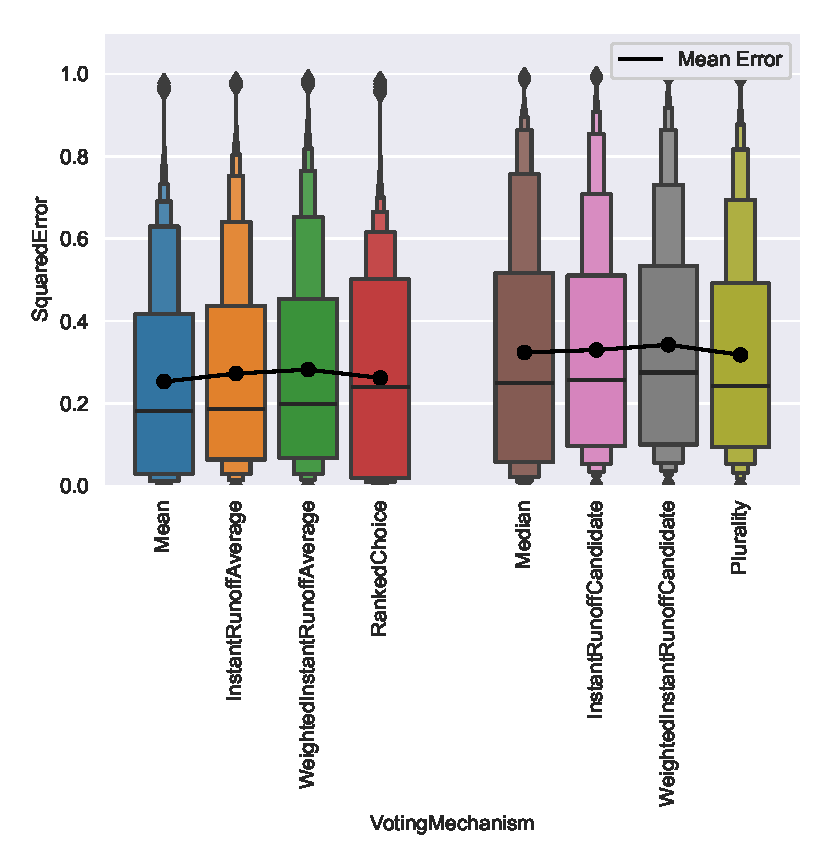
\includegraphics[scale=0.75]
    {./content/figures/voting_mechanisms/voting_mechanisms_comparison}
    \caption{Squared error populations by voting mechanism, with average
    mechanisms on the left and candidate mechanisms on the right.}
    \label{fig:voting-mechanisms-comparison}
\end{figure}

This graph immediately tells us a few things.
First, the squared error seems to be skewed, favoring numbers closer to 0.
This means there is a fairly even spread of estimates, since this is the
pattern one would expect to see from a uniform distribution of estimates.
Interestingly, however, is the majority of most error populations are
somewhere between a uniform distribution of estimates
(\autoref{fig:expected_even_distribution_squared_error}) and a normal
distribution (\autoref{fig:expected_gaussian_distribution_squared_error}).
Indeed, if the estimates are instead graphed as in
\autoref{fig:voting_mechanisms_estimate_distribution}, the distribution of estimates
is more normal than uniform.
This means most mechanisms are better at estimating \truth\ than random chance.

% TODO: Add a table with the mean error for each mechanism

Additionally, while all distributions appear generally close, there appears to be a
slight difference between average and candidate mechanisms.
This can be confirmed by comparing the average mechanisms to the candidate mechanisms
using a Mann-Whitney U-test, with the alternative being the average mechanisms'
squared error is lesser.
Performing such a test results in a p-value of 0.0, far below the $\alpha$ of 0.05.
Since candidate mechanisms can still be useful depending on the situation, both the
best average mechanisms and the best candidate mechanisms will be identified.

Further U-tests were performed, comparing each individual voting mechanism against
every other individual mechanism.
The results of this analysis can be found in
\autoref{fig:all-voting-mechanisms-p-values}, and is further segmented and discussed in
\autoref{subsec:lowest-error-average-mechanisms} and
\autoref{subsec:lowest-error-candidate-mechanisms}.

\subsection{Average Mechanisms}\label{subsec:lowest-error-average-mechanisms}
Average mechanisms, as described in \autoref{subsubsec:average-mechanisms}, work by
averaging the estimates of the system's agents, so it is not too surprising they
result in less error than candidate mechanisms which ultimately output only a single
agent's estimate.
However, they are not all created equally.
This leads us to the question: which average mechanisms generally work best?

To start, an ANOVA test was performed on the average mechanisms.
This produced a p-value of 0, indicating there is very likely a difference between
average mechanisms.
U-tests were then performed to compare each mechanism on its own against each other
mechanism individually, resulting in \autoref{fig:average-mechanisms-p-values}.
The numbers next to the edges are the resultant p-values, where the alternative is
the population is lower than the other.
As is shown by the graph, there is sufficient evidence to reject the null hypothesis
than any of the populations are the same.

\begin{figure}[htbp]
    \centering
    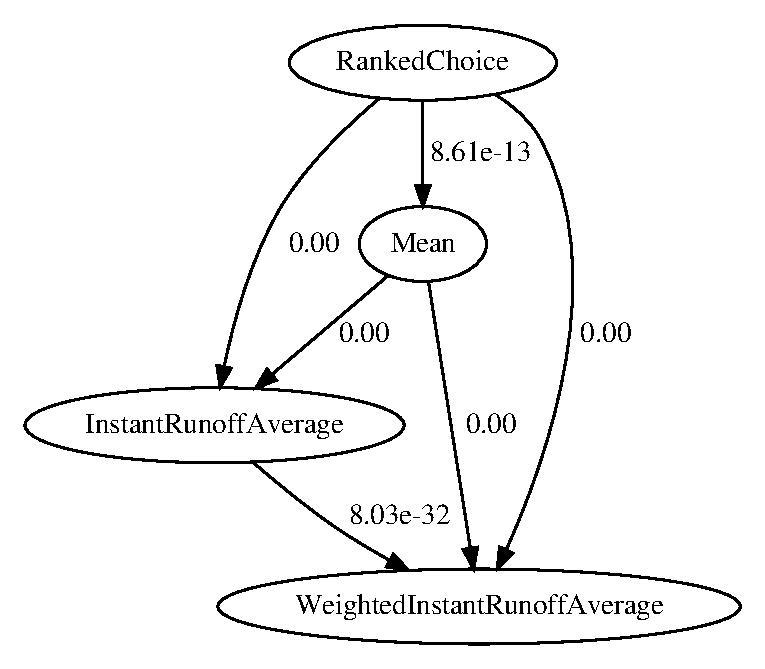
\includegraphics[scale=0.75]
    {./content/figures/voting_mechanisms/average-mechanisms-p-values.gv}
    \caption{The p-values for average voting mechanisms, given the alternative is one
    population is lesser than the other.
    An arrow pointing to another voting mechanism indicates the `from' mechanism
    beats the `to' mechanism.}
    \label{fig:average-mechanisms-p-values}
\end{figure}

In addition, Ranked Choice appears to beat out every other voting mechanism, followed
by Mean beating two, then Weight by Instant Runoff beating one, and finally Averaged
Weighted Instant Runoff beating none.
\begin{samepage}
    This means the rankings of the average mechanisms is as follows:
    \begin{enumerate}
        \item \hyperref[para:avg-ranked-choice]{Ranked Choice}
        \item \hyperref[para:mean]{Mean}
        \item \hyperref[para:avg-instant-runoff]{Weight by Instant Runoff}
        \item \hyperref[para:avg-weighted-instant-runoff]{Averaged Weighted Instant
        Runoff}
    \end{enumerate}
\end{samepage}

\subsection{Candidate Mechanisms}\label{subsec:lowest-error-candidate-mechanisms}
Candidate voting mechanisms are described in \autoref{subsubsec:candidate-mechanisms}.
They work by selecting a single `candidate' and uses its vote as \systemtruth.
While they do not appear to perform as well as average mechanisms, they may be
circumstances where they are required and so they will still be analyzed to determine
which candidate mechanism works best.

An ANOVA analysis was again used to start, which resulted in a p-value of
$2.49e-221$.
This, again, is clearly below $\alpha$, so we can reject the null hypothesis that all
populations are the same.
Following the pattern of analysis in
\autoref{subsec:lowest-error-average-mechanisms}, U-tests where then performed to
identify which mechanisms produced lower error than others.
The p-values can be found in \autoref{fig:candidate-mechanisms-p-values}.

\begin{figure}[htbp]
    \centering
    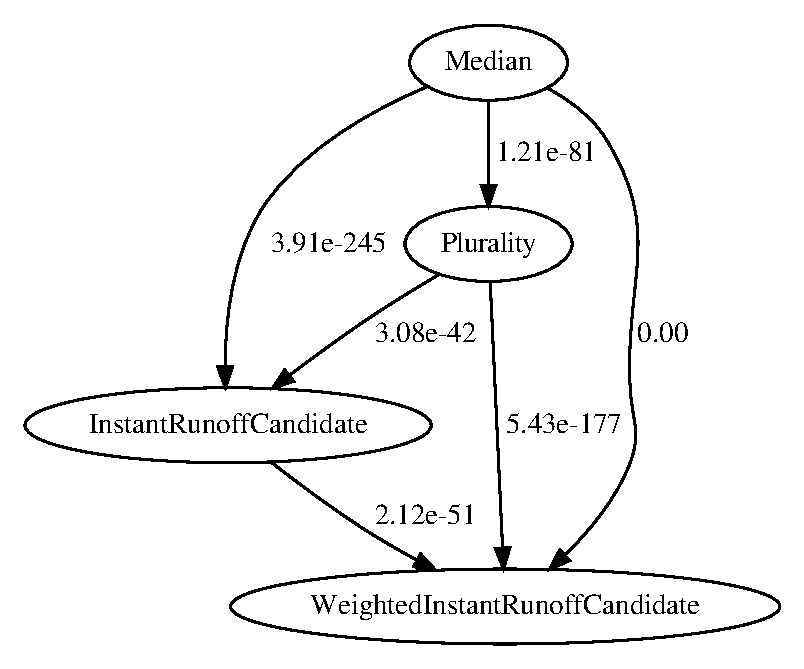
\includegraphics[scale=0.75]
    {./content/figures/voting_mechanisms/candidate-mechanisms-p-values.gv}
    \caption{The p-values for candidate voting mechanisms, given the alternative is one
    population is lesser than the other.
    An arrow pointing to another voting mechanism indicates the `from' mechanism
    beats the `to' mechanism.}
    \label{fig:candidate-mechanisms-p-values}
\end{figure}

While not as many p-values are 0 with the candidate mechanisms, there is still very
strong evidence that each candidate mechanism is not the same as each other.
For the candidate mechanisms, Median appears to be the best, followed
by Plurality, Instant Runoff, and finally Weighted Instant Runoff.
\begin{samepage}
    This means the rankings of the candidate mechanisms is as follows:
    \begin{enumerate}
        \item \hyperref[para:median]{Median}
        \item \hyperref[para:plurality]{Plurality}
        \item \hyperref[para:cand-instant-runoff]{Instant Runoff}
        \item \hyperref[para:cand-weighted-instant-runoff]{Weighted Instant Runoff}
    \end{enumerate}
\end{samepage}


\section{Lowest Error Weighting Mechanisms}\label{
    sec:lowest-error-overall-weighting-mechanism}
Weighting mechanisms have a direct influence on how voting mechanisms operate in that
they apply weights to the estimates of the proxies.
This naturally has a direct impact on the output of a system.
\autoref{fig:weighting-mechanisms-comparison}

\begin{figure}[htbp]
    \centering
    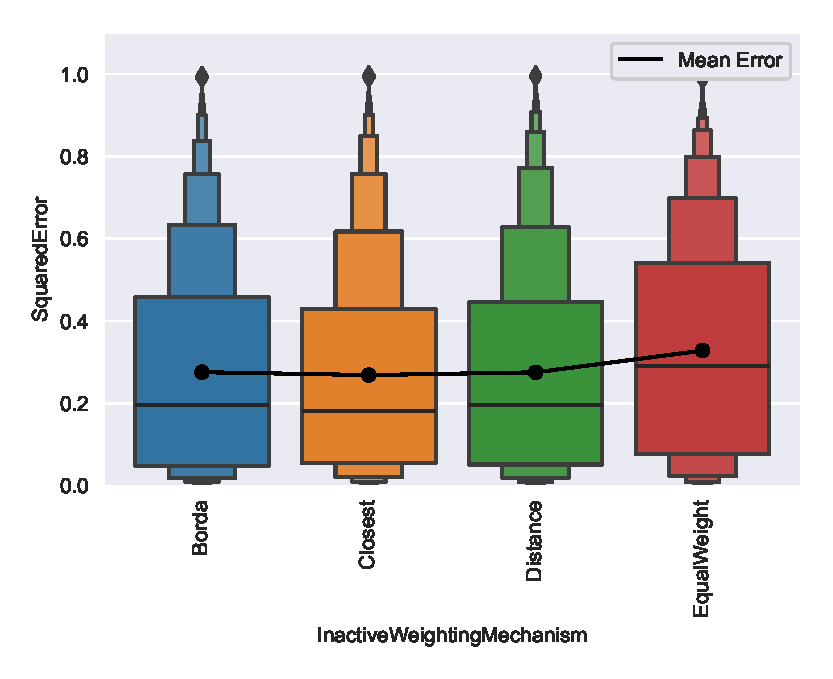
\includegraphics[scale=0.75]
    {./content/figures/weighting_mechanisms/weighting_mechanisms_comparison}
    \caption{Squared error populations by weighting mechanism.}
    \label{fig:weighting-mechanisms-comparison}
\end{figure}

% TODO: Add a table with the mean error for each mechanism

While the mechanisms definitely appear close, there is a visible difference between
the Equal Weight mechanism and the other mechanisms.
This can be confirmed using a series of Mann-Whitney U-tests, resulting in
\autoref{fig:weighting-mechanisms-p-values}.
\begin{samepage}
    This gives us the ordering:
    \begin{enumerate}
        \item \hyperref[para:closest]{Vote for Closest}
        \item \hyperref[para:borda]{Borda}
        \item \hyperref[para:distance-voting]{Distance Voting}
        \item \hyperref[para:equal-weight]{Equal Weight}
    \end{enumerate}
\end{samepage}

\begin{figure}[htbp]
    \centering
    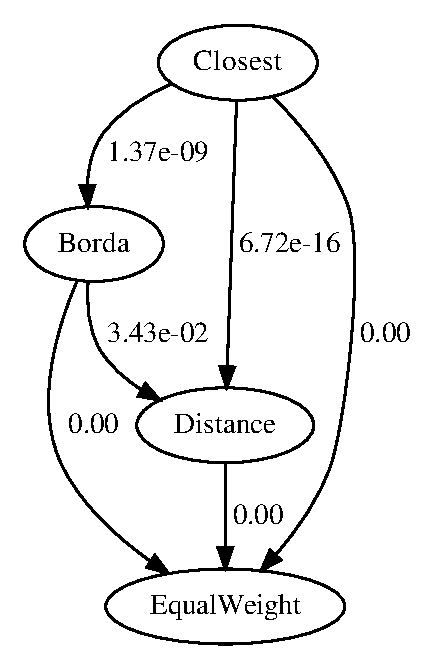
\includegraphics[scale=0.75]
    {./content/figures/weighting_mechanisms/weighting-mechanisms-p-values.gv}
    \caption{The p-values for weighting mechanisms, given the alternative is one
    population is lesser than the other.
    An arrow pointing to another voting mechanism indicates the `from' mechanism
    beats the `to' mechanism.}
    \label{fig:weighting-mechanisms-p-values}
\end{figure}

These results are somewhat surprising in that the simplest method, arguably barring
Equal Weight, appears to produce the best results.
This may be due to the Closest mechanism yielding a lower system-wide weight while
still maintaining an ordering of preferences.
However, this does not necessarily mean the Closest mechanism pairs best with all
voting mechanisms.
This idea is explored in~\fullref{sec:lowest-error-overall-combination}.


\section{Lowest Error Combination}\label{sec:lowest-error-overall-combination}


\section{Best Inactive to Proxy Ratio}\label{sec:best-inactive-to-proxy-count}


\section{Caveat}\label{sec:caveat}
% Explain how WeightlessAverageAll works best
% TODO: Try to find some cirumstance where some else works better

